\chapter{引言}
\label{cha:intro}


\section{研究背景}

从古至今,信息的主要交流方式是基于语言的,人类知识的长期传承也是通过语言文字这个载体进行下去的。可以说,从人类早期的莎草纸、羊皮卷、竹简到之后的纸张,上面的文本内容成了知识千年以来突破时空的重要途径。而伴随着互联网在二十一世纪的蓬勃发展,信息的传递速度、传递带宽、一次载体能够传递的信息量都得到了极大提升。信息的增长趋势也从过去的线性级别增长变成了指数级别的增长,这意味着每天都有成千上万的信息涌入了网络之中。这些海量的数据一方面使得信息的来源变的空前丰富,但同时也使得我们对信息的把握、筛选遇到了巨大障碍。信息爆炸同时伴随噪音爆炸,在这样的环境下,从海量的嘈杂的文本中提取知识是不容易的。在这样的背景下,为了有效地获取知识,知识图谱(KG)的概念被提出并在学术界和工业界都受到了广泛的关注。

知识图谱(Knowledge Graph, KG),某些场景下也被称为知识库(Knowledge Base,KB),是一种将现实世界中人类的知识结构化之后形成的知识系统。在知识图谱中,大量的知识,诸如开放数据库和百科全书中的信息,通常以关系数据集合的形式被表达出来。而在关系数据集合中,基本事实被抽象为实体(Entity),而规则、逻辑、推理等关联性的信息则被抽象为实体间的关系(Relation)。若将实体对应于点,关系对应于边,则这些知识可以进一步以图的形式呈现,从而可以被计算机高效的使用,而这也是研究知识图谱的意义所在。这种将实体和抽象概念结构化成多关系数据库的模式也是近年来被大力提倡的,我们接触到的信息,尤其是文本信息突破了以往字符串线形构成的基本形式,可以以实体和关系构成的网状形式存在。

目前知识图谱已经作为人工智能领域的一项基础核心技术,被广泛引入到信息检索(Information Retrieval,IR)、问答系统(Question Answering,QA)、推荐系统(Recommender System,RS)等任务上。图谱中优质的结构化知识信息,能够指导我们的智能模型具备更深层的事物理解、更精准的任务查询以及可能的逻辑推理能力,从而在这些知识驱动应用中起着至关重要的作用。可以毫不夸张的说,正是由于这些结构化知识图谱的存在,我们建模实体以及实体之间的关系变的容易,让计算机能够理解知识、运用知识甚至于发掘创造知识的想法也逐渐具有了可行性。

\vspace{25pt}
\begin{figure}[!htbp]
\setlength{\abovecaptionskip}{30pt} 
\centering
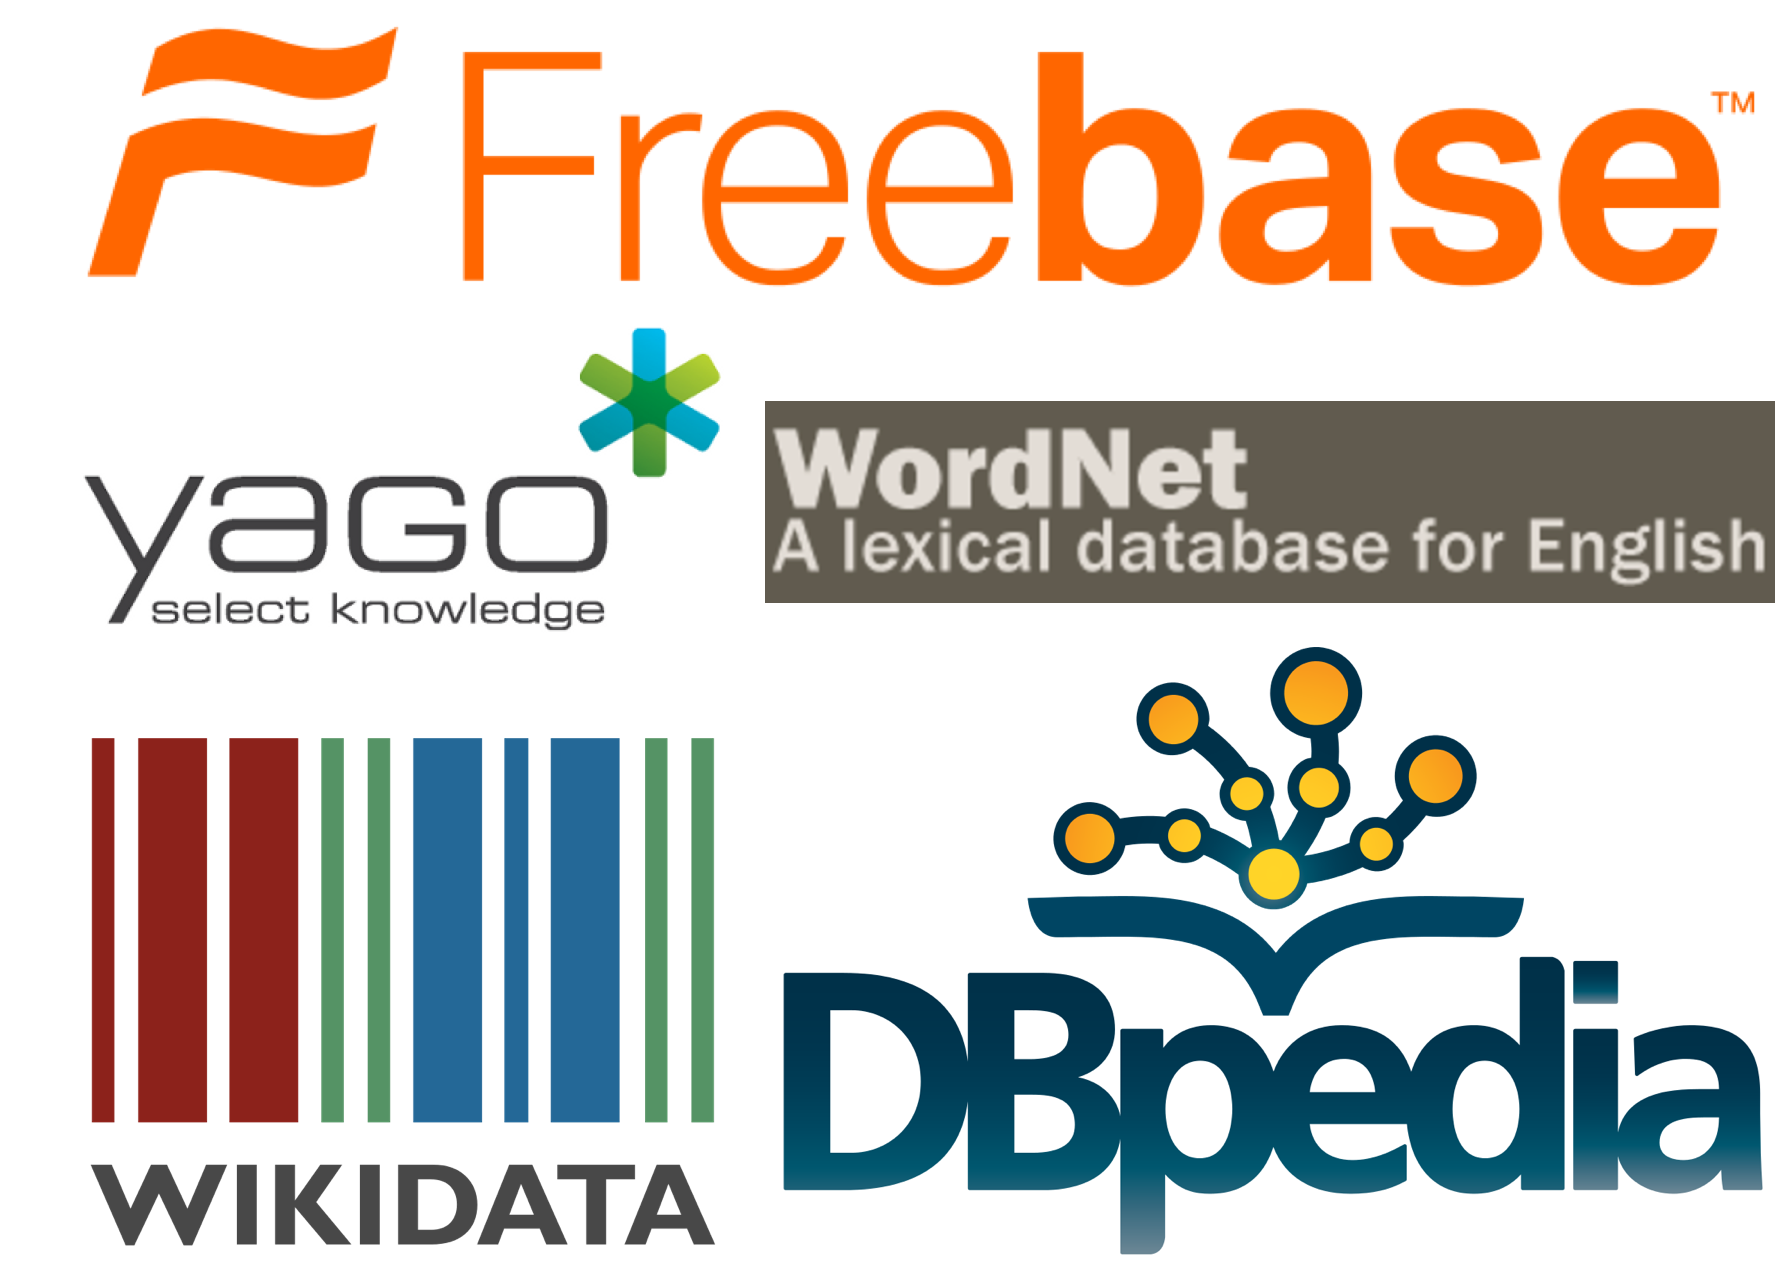
\includegraphics[width=0.8\columnwidth]{figures/ch1/KG_example.png}
\caption{一些常用的大规模知识图谱}
\label{ch1:KG_example}
\end{figure}

而随着时间的积累和相关工作者长期的工作,结合机器自动标注、专家标注和开放平台编辑校对等多种方法,现在已经构建出一些诸如图\ref{ch1:KG_example}中的高质量的大规模知识图谱,诸如 WordNet \cite{miller1995wordnet},YAGO \cite{hoffart2013yago2},DBPedia \cite{auer2007dbpedia},Freebase \cite{bollacker2008freebase},Wikidata \cite{vrandevcic2014wikidata} 以及 Knowledge Vault \cite{dong2014knowledge},并且被投入到部分相关研究场景中。截止到Freebase停止更新为止,Freebase中收集了超过 $2$ 亿个的实体,在其停止维护后这些信息正在被陆续迁移到 Knowledge Vault 和 Wikidata 中。经过维基社区的过滤和校对,截止目前,Wikidata中也有超过 $2600$ 万个高质量实体存在。与此同时,国内从事互联网领域尤其是和信息检索直接相关的企业也对知识图谱进行了投入,百度知心和搜狗知立方作为典型的中文知识图谱被构建出来并被使用到智能应用产品中进行知识驱动。

知识图谱将具象事物与抽象概念表示为实体,将实体之间的联系表示为关系,并以( \emph{头实体}, \emph{关系}, \emph{尾实体} )的形式表述知识。例如,“马克·吐温出生于佛罗里达州”在知识图谱中被表述为( \emph{马克·吐温}, \emph{出生于}, \emph{佛罗里达州} );“北京市下辖海淀区”在知识图谱中被表述为( \emph{北京市}, \emph{区划管辖}, \emph{海淀区} )等等。其中\emph{马克·吐温}、\emph{佛罗里达州}、\emph{北京市}、\emph{海淀区}即为实体,而\emph{出生于}、\emph{区划管辖}则是实体间的关系。一般来说,现在公开的知识图谱都是以这样的事实三元组(triple fact)的 形式抽象知识,并采用类似于万维网联盟(W3C)发布采用的资源描述框架(Resource Description Framework, RDF)进行储存。图\ref{ch1:google_kg_example}中展现的就是使用谷歌搜索``北京''时弹出的相关知识图谱。

\vspace{25pt}
\begin{figure}[h]
\setlength{\abovecaptionskip}{30pt} 
% \setlength{\textfloatsep}{60pt} 
\centering
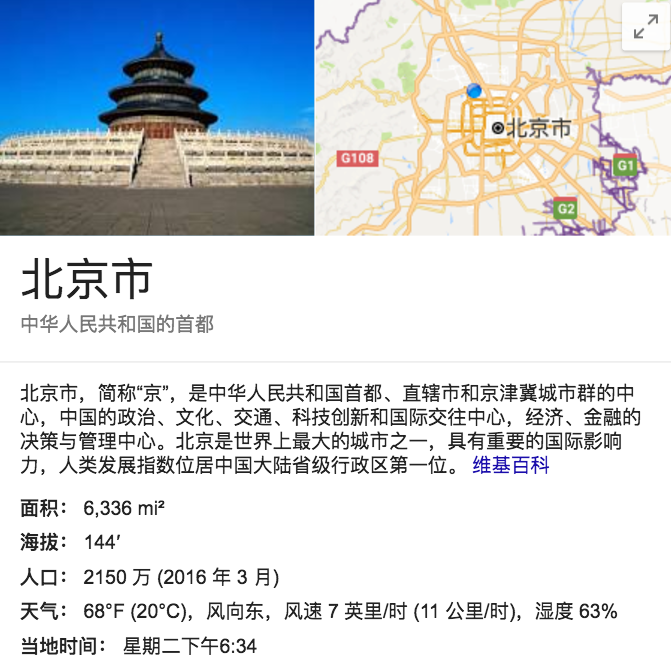
\includegraphics[width=0.6\columnwidth]{figures/ch1/knowledge.png}
\caption{日常搜索中出现的知识图谱}
\label{ch1:google_kg_example}
\end{figure}

伴随着上个世纪末互联网的蓬勃发展以及本世纪初信息技术的大量普及,在大量知识被整理进入知识图谱的同时,每天也有大量的知识产生。虽然当前的知识图谱离完善还差的很远,但以结构化形式存在于知识图谱中的知识也是相当惊人的多。而伴随着信息爆炸式增长以及日新月异的变化,海量的数据如何整理、存储、更新以及应用都是巨大的挑战。而这些知识图谱带来的技术诉求,其中很重要的一点就是如何以一个高效的方式进行知识图谱的表示。基于事实三元组集合的形式来表示知识图谱可以解决底层数据存储形式的问题,这与关系数据库的模式是十分相似的。但这样简单的抽象形式对于理解图谱、应用图谱乃至于依靠知识进行逻辑推理确是远远不够的。想要以高效的形式对知识图谱进行更高层的抽象,并且能够做到利用知识,这其中面临着许多难题:其一,是在计算效率上的问题。知识图谱往往以有向图的形式存在,以点为实体边为关系,这样的形式简单明了,却也需要图相关的算法来进行处理。早期基于图结构的图谱表示算法,其计算复杂度通常都非常高,以至于在大规模的知识图谱上难以适用。其二,知识图谱中实体和关系都很多,却没有实体数平方级别的事实三元组,这意味着知识图谱是稀疏图而非稠密图。与此同时,实体之间也相差很大,满足幂律分布。少部分高频实体和关系涵盖了多数的事实三元组,其余均是长尾部分。数据的稀疏性以及长尾分布也为模型设计带来巨大难度。

\vspace{25pt}
\begin{figure}[h]
\setlength{\abovecaptionskip}{30pt} 
\centering
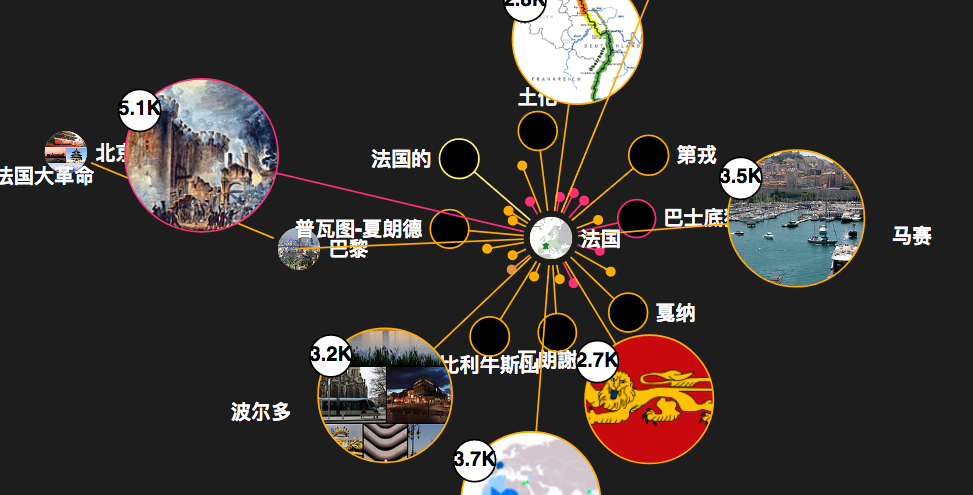
\includegraphics[width=0.9\columnwidth]{figures/ch1/space.png}
\caption{BabelNet 中与实体``法国''空间距离最近的实体}
\label{ch1:space}
\end{figure}

研究和解决抽象知识图谱过程中的计算复杂度与数据稀疏性问题,并将知识图谱表达为计算机可使用的模式,就是知识表示学习(Knowledge Representation Learning, KRL)的主要任务。近些年来,受到文本词向量的启发,将图谱进行分布式表示逐渐成为趋势。对于知识图谱来说,所谓的分布式表示(Distributed Representation),其实质就是将图谱中的实体和关系映射到低维度的连续空间中去。在映射空间上,对象之间的距离关系可以直接反映语义关联,比如语义相似的实体,其空间距离一般都十分相近。图\ref{ch1:space}展现的就是空间上与``法国''最相关的实体,数据来源于 BabelNet \footnote{http://babelnet.org/}。因为这个过程实际是将实体与关系的语义信息嵌入到低维度空间上,所以我们通常也将这个过程称为嵌入,得到的向量称为嵌入表示或直接称为嵌入(Embedding)。分布式表示一定程度上解决了之前提到的问题:首先,将知识图谱嵌入到低维度空间上,低维度的空间让实体与关系之间的语义关联计算更加便利,计算量也显著减少。其次,赋予每个实体与关系实数向量的表示,并且向量之间的空间关系来表示语义关联,很大程度上让知识图谱的分布不再稀疏。最后,以数值形式存在的知识图谱对于计算机来说比字符更容易理解和计算,将其作为其他各个应用模型的输入也变的容易起来。得益于知识表示学习在分布式表示上的有效推进,相关领域的工作也不断推陈出新,涌现了一批知识驱动为内核的模型。

虽然在知识表示学习的研究中已经有大量优秀的模型出现,且在实验数据集合上体现出了良好的性能。但是在实验环境中,数据集往往与实际的知识图谱相差甚远,通常只是公开大规模知识图谱的子集。通过实际对比可以发现,大规模的知识图谱无论在规模还是在分布上都比实验数据集合难处理的多,呈现出规模巨大、长尾突出的状态。与此同时,实验过程中模型的设计在突出性能考虑的时候往往忽略了模型复杂度,其工程实现也难以承受巨大规模的数据量。另一方面,知识图谱常常会与多源信息进行融合,尤其是与自由文本进行融合。以往的知识图谱与文本的融合模型均以串行形式进行融合,这也是很难在极大数据量的背景下进行训练与处理的。本文工作的主要目的就是立足于现有模型的基础上提出一套针对大规模知识图谱的表示学习框架、特征融合框架,在真实的大规模知识图谱上进行训练并得到优质的嵌入表示。

\section{相关资源}


 % \footnote{WordNet: http://wordnet.princeton.edu/ \\ YAGO: http://www.mpi-inf.mpg.de/departments/databases-and-information-systems/research/yago-naga/yago/ \\ DBPedia: http://wiki.dbpedia.org/ \\ Freebase: https://developers.google.com/freebase/ \\ Wikidata: https://www.wikidata.org/wiki/Wikidata:Main\_Page/} 


\section{研究内容}

\section{本文贡献}

  本文贡献总结如下:

  (1)通过底层实现的优化以及对知识图谱的划分,将以往的图谱模型改造成基于多线程的训练模型,在未来可以进一步衍生为分布式的训练模型,从而能够高效的对大规模知识图谱进行学习。
  
  (2)提出了加权点采样算法和位移负样例采样算法来取代原有的边采样及负例采样算法。能够在大规模图谱的幂率分布下对图中不同的实体和事实赋予不同的注意度,缓解幂率分布带来的长尾影响。二点采样的训练方式,可以在训练过程中尽可能的合并算术运算从而进一步加速。
  
  (3)采用了平行结合的方式与文本神经网络模型融合,对比于传统的串行结合方式,这样的模型能够更快的引入文本信息来丰富图谱内容并进行信息融合。在此基础上我们提出了一套联合学习的方法,使得图谱和文本的信息融合是双向的,图谱和文本模型融合之后两者都有显著效果提升
  
  (4)本文的相关工作提供了开源代码并对之前领域内的相关工作进行整理和总结,为之后相关领域需要使用知识图谱的后续研究打好基础,提供便利。

\section{论文组织}

  本文在第二章中综述知识图谱的发展轨迹,并对已有的知识图谱表示学习模型进行介绍、分析,从而能够对这一任务的相关工作进行梳理和总结。第三章介绍过去几年中被提出的知识图谱和文本模型的结合方法及相关任务,其中重点综述神经网络引入后深度模型的发展和联合学习模型的发展。第四章介绍我们提出的在大规模知识图谱背景下进行表示学习的框架,以及在此框架下和文本部分进行并行融合的联合学习方法。第五章介绍实验所用的数据并给出量化的评测结果,验证本文提出框架的准确性、可靠性和运行效率。
